\documentclass[12pt]{article}

\setlength{\parindent}{0em}
\setlength{\parskip}{.5em}

\usepackage{framed}
\newcounter{problem}
\newcounter{problempart}[problem]
\newcounter{solutionpart}[problem]
\newenvironment{problem}{\stepcounter{problem}\noindent{\bf\arabic{problem}.}}{\setcounter{problempart}{0}\setcounter{solutionpart}{0}}
\newenvironment{solution}{\par\textcolor{green!50!black}\bgroup}{\egroup\par}
\newcommand{\qpart}{\stepcounter{problempart}${}$\\\noindent{(\alph{problempart})} }
\newcommand{\spart}{\stepcounter{solutionpart}${}$\\\noindent{(\alph{solutionpart})} }
\newcommand{\TODO}{\textcolor{red}{$\blacksquare$}}

\usepackage{hyperref}
\usepackage{fullpage}
\usepackage{amsmath,mathabx,MnSymbol}
\usepackage{color,tikz}
\usepackage{pstricks}
\usepackage{pst-plot,pst-node}
\usepackage{footnote,enumitem}
\usepackage{longtable}
\newcommand{\mx}[1]{\begin{pmatrix}#1\end{pmatrix}}
\definecolor{dkgreen}{rgb}{0,.5,0}
\usepackage{algorithm}
\usepackage[noend]{algpseudocode}

\newcommand{\uu}{\mathbf{u}}
\newcommand{\vv}{\mathbf{v}}
\newcommand{\cc}{\mathbf{c}}
\newcommand{\ww}{\mathbf{w}}
\newcommand{\xx}{\mathbf{x}}
\newcommand{\zz}{\mathbf{z}}
\newcommand{\ee}{\mathbf{e}}
\newcommand{\pp}{\mathbf{p}}
\newcommand{\qq}{\mathbf{q}}
\renewcommand{\AA}{\mathbf{A}}
\newcommand{\BB}{\mathbf{B}}
\newcommand{\nn}{\mathbf{n}}
\newcommand{\gp}[1]{\left(#1\right)}

\newcommand{\TODOL}[1]{\textcolor{red}{\underline{\hspace{#1 cm}}}}

\usepackage{listings}

\lstset{
  language=C++,
  showstringspaces=false,
  identifierstyle=\color{magenta},
  basicstyle=\color{magenta},
  keywordstyle=\color{blue},
  identifierstyle=\color{black},
  commentstyle=\color{green},
  stringstyle=\color{red}
}

\begin{document}

\title{CS130 - LAB - Bresenham's line algorithm / midpoint algorithm}
\date{}
\author{Name: \TODOL7\qquad\qquad SID: \TODOL4}
\maketitle
\begin{center}
\end{center}

\section*{Part 1: Bresenham's line algorithm / midpoint algorithm}

References: \href{https://en.wikipedia.org/wiki/Bresenham%27s_line_algorithm}{https://en.wikipedia.org/wiki/Bresenham\%27s\_line\_algorithm}

This Lab consists of implementing the midpoint algorithm to draw continuous
lines using only integer operations. Recall the line equation is $y = mx + n$,
where $m$ is the slope and $n$ is the $y$ intercept.  Given two points $p_0 =
(x_0, y_0)$ and $p_1 = (x_1, y_1)$, the slope is calculated as $m = \frac{y_1 -
  y_0}{x_1 - x_0} = \frac{dy}{dx}$.  Consider $0 \le m \le 1$ (line in angle
between 0 and 45 degrees).  The idea is to determine which of the two pixels
($a$ or $b$) we should draw. Complete the missing coordinates of the points
below.\\
\begin{center}
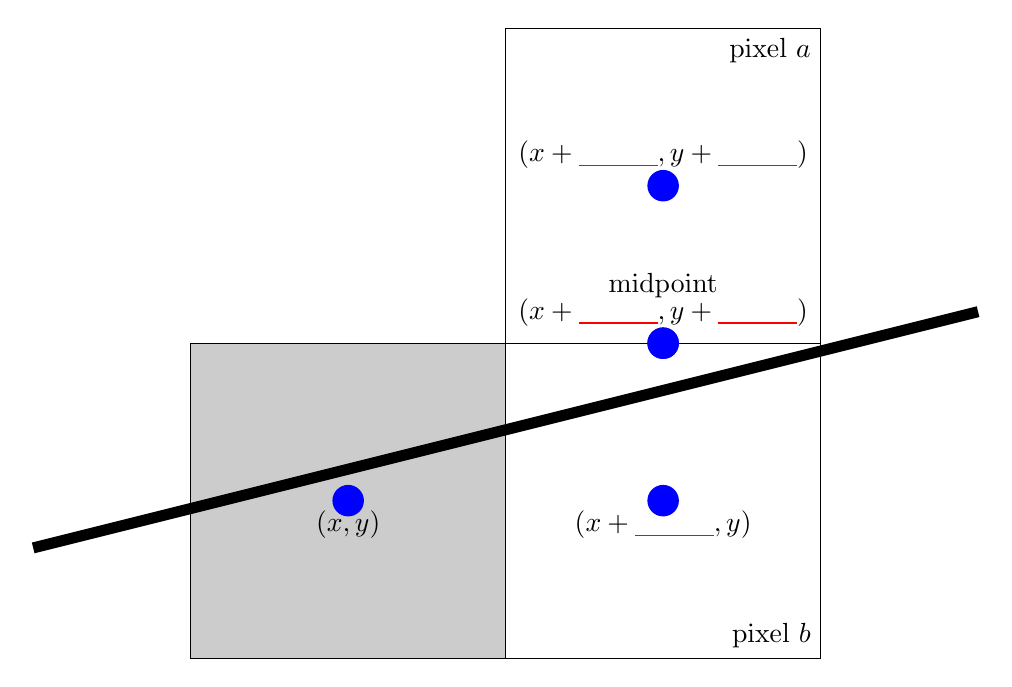
\begin{tikzpicture}[scale=2]
\draw[fill=black!20] (0,0) rectangle (2,2);
\draw[] (2,0) rectangle (4,2);
\draw[] (2,2) rectangle (4,4);
\draw[fill=blue,draw=none] (1,1) node[below]{$(x,y)$} circle (.1);
\draw[fill=blue,draw=none] (3,1) node[below]{$(x+\TODOL1,y)$} circle (.1);
\draw[fill=blue,draw=none] (3,3) node[above,inner sep=6]{$(x+\TODOL1,y+\TODOL1)$} circle (.1);
\draw[fill=blue,draw=none] (3,2) node[above,inner sep=6]{$(x+\TODOL1,y+\TODOL1)$} circle (.1);
\draw[fill=blue,draw=none] (3,2) node[above,inner sep=6+1em]{midpoint} circle (.1);
\node[above left] at (4,0) {pixel $b$};
\node[below left] at (4,4) {pixel $a$};
\draw[line width=4] (-1,.7) -- (5,2.2);
\end{tikzpicture}
\end{center}

In particular, we can evaluate the midpoint between $a$ and $b$ using a function
$f(x,y)$ that returns a positive number if the line is above the midpoint and
negative if the line is below the midpoint.  The function $f(x,y)$ should be
zero if the midpoint lies on the line
\begin{align}\label{eqn:fxy}
f(x, y) = 0 = mx + n - y
\end{align}
Rewrite the right-hand-side (RHS) of Equation (\ref{eqn:fxy}) in the form $Ax +
By + C$, where $A$, $B$, and $C$ depends on $dx$, $dy$ and $n$ only. Remove any
denominator by multiplying $f(x, y)$ by $dx$ to ensure we have an integer
solution.
\begin{align}\label{eqn:fxy2}
  f(x, y) = \TODOL4
\end{align}
where $A = \TODOL3, B = \TODOL3, C = \TODOL3$

We want to make a decision on whether to draw pixel $a$ or $b$ using $f(x, y)$ on a
sequence of points from $p_0$ to $p_1$. Define variables $da$ and $db$ to hold
the difference of $f(x, y)$ from $a$ and $b$ to the previous midpoint $(x + 1, y
+ 1/2)$. Use Equation (\ref{eqn:fxy2}) to rewrite Equations (\ref{eqn:da}) and
(\ref{eqn:db}) as function of $A$ and $B$ (you won't need $C$).
\begin{align}
da &= f(x + 2, y + 3/2) - f(x + 1, y + 1/2) = \TODOL4 \label{eqn:da}\\
db &= f(x + 2, y + 1/2) - f(x + 1, y + 1/2) = \TODOL4 \label{eqn:db}
\end{align}
Final detail, we need to calculate the difference between the second
and first point in order to use Equations (\ref{eqn:da}) and (\ref{eqn:db}) in a loop.
\begin{align}\label{eqn:dinit}
dinit = f(x0 + 1, y0 + 1/2) - f(x0, y0) = \TODOL4
\end{align}
We only care whether $d$ is positive or negative, hence, we can multiply
$dinit$, $da$ and $db$ by 2 to get equations containing only integers.

Using Equations (\ref{eqn:fxy2}) to (\ref{eqn:dinit}), complete the midpoint
algorithm below:
\begin{lstlisting}
MPA(x0, y0, x1, y1):
  dx = x1 - x0
  dy = y1 - y0
  D = (              ) // initialize D using dinit
  y = y0
  for x = x0 to x1:
    set_pixel(x, y)
    if D > 0:
       y = y + 1
       D = (             ) // D is positive, use da
    D = (           ) // D is negative, use db
\end{lstlisting}

\section*{Part 2: Implementing the midpoint algorithm}

We considered $0 \le m \le 1$ (line in angle between 0 and 45 degrees) to write
the code in the previous part. How can we manage other angles? Feel free to
think a little bit about it and to look at the Wikipedia page (link on Part
1). Here is a free blank space and a diagram.

\begin{center}
  \begin{tikzpicture}[scale=1]
    \draw[very thick] (-4,0) -- (4,0);
    \draw[very thick] (0,-4) -- (0,4);
    \draw[very thick,dotted] (-4,-4) -- (4,4);
    \draw[very thick,dotted] (-4,4) -- (4,-4);
    \node[] at (3,1) {$0 < m < 1$};
    \node[] at (1,3) {$m > 1$};
    \node at (5,2.5) {$1^{\mbox{st}}$ quadrant};
    \node at (5,2) {$x_0 < x_1$, $y_0 < y_1$};
    \node at (-5,2.5) {$2^{\mbox{nd}}$ quadrant};
    \node at (-5,2) {$x_0 < x_1$, $y_0 < y_1$};
  \end{tikzpicture}
\end{center}

Download the skeleton code on the website and write the midpoint algorithm in
the function \texttt{draw\_line\_MPA} in \texttt{application.cpp}.  To draw a
pixel, you can use \texttt{set\_pixel(x, y, linecolor)}, where linecolor is
given to you as argument of \texttt{draw\_line\_MPA}.  The following commands
are available:

\begin{itemize}
\item
  {Click and hold to draw lines.}
\item
  {Type ``c''to clear old lines.}
\item
  {Type ``a''to generate 1K random lines.}
\item
  {Type ``A''to generate 1M random lines.}
\item
  {Type ``m''to toggle between the MPA and the DDA algorithms.}
\item
  {Type ``[''or ``]''to change point-size.}
\end{itemize}

Make sure your code runs faster than the DDA algorithm. Why is the DDA algorithm
slower? Feel free to take a look at \texttt{draw\_line\_DDA} code.

Run your MPA algorithm 3 times with 1K and 1M lines without increasing the
point-size. Run the DDA algorithm 3 times with 1K and 1M lines without
increasing the point-size. Fill the table below with the running time.

DDA (1K / 1M): Run 1 = \TODOL1/\TODOL1; Run 2 = \TODOL1/\TODOL1; Run 3 = \TODOL1/\TODOL1\\
MPA (1K / 1M): Run 1 = \TODOL1/\TODOL1; Run 2 = \TODOL1/\TODOL1; Run 3 = \TODOL1/\TODOL1

\end{document}
